\documentclass[11pt]{article}
\usepackage[margin=1in]{geometry}
\usepackage{amsmath,amssymb,amsthm,graphicx,booktabs,multirow,threeparttable,setspace,array}
\usepackage[round]{natbib}
\usepackage[hidelinks]{hyperref}
\usepackage{caption,enumitem,tikz,pgfplots}
\usetikzlibrary{positioning}
\pgfplotsset{compat=1.17}
\definecolor{npblue}{RGB}{31,78,121}
\definecolor{npmid}{RGB}{72,120,168}
\definecolor{gred}{RGB}{176,74,74}
\definecolor{gold}{RGB}{200,162,74}
\captionsetup{font=small,labelfont=bf}
\setstretch{1.3}
\newcommand{\VaR}{\mathrm{VaR}}
\newcommand{\ES}{\mathrm{ES}}
\newtheorem{proposition}{Proposition}
\newtheorem{lemma}{Lemma}
\renewcommand{\thefigure}{OA.\arabic{figure}}
\renewcommand{\thetable}{OA.\arabic{table}}
\renewcommand{\thesection}{OA.\arabic{section}}
\title{Online Appendix\\ \large Semiparametric Value-at-Risk and Expected Shortfall with a Real-Time Misspecification Score}
\author{Sean Qin \and Wenxin Jiang}
\date{\today}
\begin{document}
\maketitle
\section{Algorithms}
\medskip\noindent\fbox{\parbox{0.96\textwidth}{
\textbf{Algorithm OA.1 (amortized shape model).}
(i)~Assemble the pooled panel $\{(s_{j,t}, \widehat{z}_{j,t})\}$ over
names $j$ and days $t$.
(ii)~Train $H_\phi$ by SGD on
$\mathbb{E}_{\tau\sim\lambda}\,\rho_\tau(\widehat{z} - H_\phi(s,\tau))$
[network], or boost per-$\tau$ regressions on a grid [trees]; enforce
monotonicity by rearrangement.
(iii)~For any asset, including one with no return history, using characteristics-only $s$, evaluate $H_\phi(s_t,\cdot)$; no per-asset
estimation step exists.
(iv)~To \emph{sample}, draw $\tau^{(m)}\sim U(0,1)$ and return
$z^{(m)} = H_\phi(s_t,\tau^{(m)})$.
}}

\medskip\noindent\fbox{\parbox{0.96\textwidth}{
\textbf{Algorithm OA.2 (the misspecification meter, as deployed).}
(i)~Fit equation~(1) of the paper on a trailing window; store
$\widehat{z}_{t-62},\dots,\widehat{z}_t$.
(ii)~Compute $\mathrm{mk}_{63}$, $|\mathrm{sk}_{63}|$, $J_5$ by
equation~(12) of the paper.
(iii)~Convert each to its percentile against the trailing pooled panel
(same asset class); the score is the maximum of the three percentiles,
re-ranked into deciles.
(iv)~Act by the paper: top decile $\Rightarrow$ the parametric
model's average pinball loss runs $\sim$2--3\% higher within this
score region (a conditional average, not a per-name point estimate), flag the asset for the nonparametric /
residual-hybrid engine and for model-risk review; elsewhere
$\Rightarrow$ no action (in the amortized setting the engine is run
regardless; the meter serves surveillance, and day-level switching is
unsupported, Section~5.4 of the paper).
(v)~Latency: detection lags episode onset by median 0 / mean 2--4 days;
the edge is back-loaded within episodes, so the lag forfeits little.
}}

\medskip\noindent\textbf{Deployed pipeline.} Each day: (i)~update each name's GARCH filter state
$\widehat\sigma_{t+1}$ (recursion only; parameters refit annually);
(ii)~assemble the state vector $s_t$ and evaluate the shared shape model $q_\phi(\tau\mid s_t)$, one model for the whole book, no
per-name estimation; (iii)~apply the frozen GPD tail below $p_0$
and, where the desk elects the coverage overlay, the conformal shift
$c_\tau$ (static or adaptive); (iv)~report
$\widehat Q_{t+1}(\tau) = \widehat\sigma_{t+1}\,\widetilde q(\tau\mid s_t)$
at the desk's levels, with VaR and ES$_{97.5}$ both read from the coherent
min-envelope curve $Q^{*}=\min\{$body$,$EVT$\}$ (VaR at the $\alpha$
node, ES its numerical tail integral); (v)~read
the misspecification score equation~(12) of the paper as the model-risk monitor: top decile means the parametric fallback's conditional average loss
in that score region runs $\sim$2--3\% higher. \emph{Annually:} refit filters, retrain the shape model,
re-estimate tail and shifts, all on trailing data. \emph{New listing:}
run the separate characteristics-only amortized forecaster until an
own-history sample sufficient to initialize the per-name scale filter
accrues; then attach this residual-hybrid pipeline. Total marginal
cost per name per day: one filter update and
one model evaluation.

\section{Supplementary figures}
% order fixes numbering: OA.1 timing, OA.2 passrates, OA.3 horizon, OA.4 frtb, OA.5 universes, OA.6 frontier
\begin{figure}[htbp]
\centering
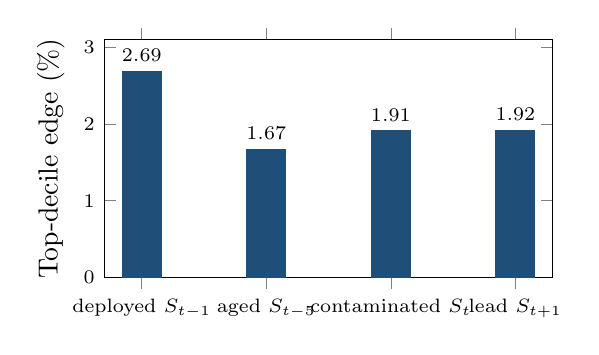
\begin{tikzpicture}
\begin{axis}[width=0.6\textwidth, height=4.6cm, ybar, bar width=14pt,
  symbolic x coords={deployed $S_{t-1}$, aged $S_{t-5}$, contaminated $S_t$, lead $S_{t+1}$},
  xtick=data, ymin=0, ymax=3.1, ylabel={Top-decile edge (\%)},
  x tick label style={font=\scriptsize}, tick label style={font=\scriptsize},
  nodes near coords, every node near coord/.append style={font=\scriptsize}]
\addplot[fill=npblue, draw=npblue] coordinates
  {(deployed $S_{t-1}$,2.69) (aged $S_{t-5}$,1.67) (contaminated $S_t$,1.91) (lead $S_{t+1}$,1.92)};
\end{axis}
\end{tikzpicture}
\caption{Timing diagnostics for the frontier. Top-decile edge under four
alignments of the mk$_{63}$ score with the daily loss (200 CRSP names;
per-date DM 5.5--6.5 in all four). The deployed lag dominates, and the
contaminated same-day alignment yields less, the opposite of what a look-ahead artifact would produce.}
\label{fig:timing}
\end{figure}
\clearpage
\begin{figure}[htbp]
\centering
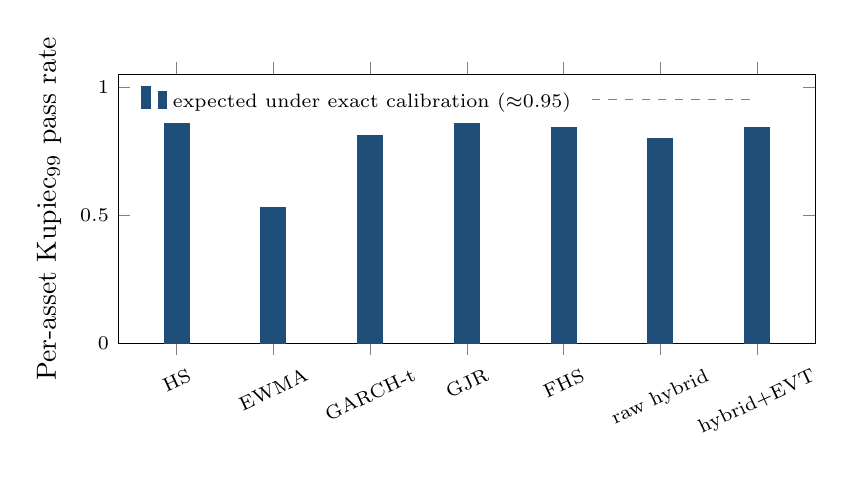
\begin{tikzpicture}
\begin{axis}[width=0.86\textwidth, height=5cm, ybar, bar width=9pt,
  symbolic x coords={HS, EWMA, GARCH-t, GJR, FHS, raw hybrid, hybrid+EVT},
  xtick=data, ymin=0, ymax=1.05, ylabel={Per-asset Kupiec$_{99}$ pass rate},
  x tick label style={font=\scriptsize, rotate=25}, tick label style={font=\scriptsize},
  legend style={font=\scriptsize, at={(0.02,0.98)}, anchor=north west, draw=none}]
\addplot[fill=npblue, draw=npblue] coordinates
  {(HS,0.93) (EWMA,0.53) (GARCH-t,0.81) (GJR,0.86) (FHS,0.84) (raw hybrid,0.80) (hybrid+EVT,0.84)};
\addplot[dashed, sharp plot, gray, mark=none] coordinates {(HS,0.95) (hybrid+EVT,0.95)};
\addlegendentry{expected under exact calibration ($\approx$0.95)}
\end{axis}
\end{tikzpicture}
\caption{Exception tests restated per asset (140 CRSP names, 99\% VaR):
share of names whose individual Kupiec test is consistent with nominal.
HS over-covers (conservative); EWMA fails; the EVT-tailed engine matches
the parametric benchmarks while beating them on loss and the joint
FZ0 score
(Table~6 of the paper). Date-clustered tests in the table notes.}
\label{fig:passrates}
\end{figure}
\clearpage
\begin{figure}[htbp]
\centering
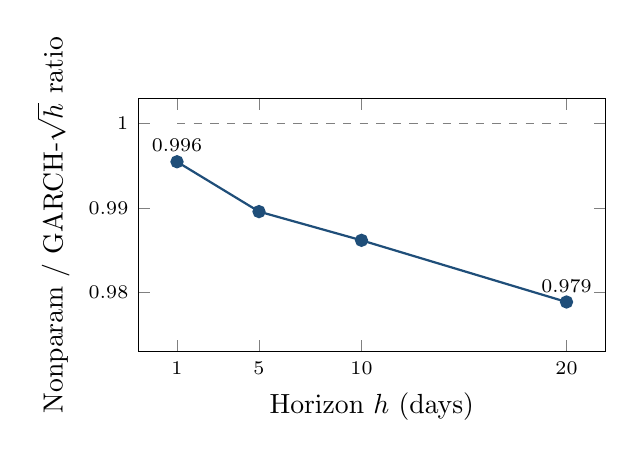
\begin{tikzpicture}
\begin{axis}[width=0.62\textwidth, height=4.8cm,
  xlabel={Horizon $h$ (days)}, ylabel={Nonparam / GARCH-$\sqrt{h}$ ratio},
  xtick={1,5,10,20}, ymin=0.973, ymax=1.003,
  tick label style={font=\scriptsize}]
\addplot[color=npblue, mark=*, thick] coordinates
  {(1,0.9955) (5,0.9896) (10,0.9862) (20,0.9789)};
\addplot[dashed, gray, mark=none] coordinates {(1,1) (20,1)};
\node[font=\scriptsize, anchor=south] at (axis cs:20,0.9789) {0.979};
\node[font=\scriptsize, anchor=south] at (axis cs:1,0.9955) {0.996};
\end{axis}
\end{tikzpicture}
\caption{The edge grows with horizon. Direct-model/GARCH pinball
ratio at $h = 1, 5, 10, 20$ days (150-name design panel; training
labels whose $h$-day window crosses the split are purged): fat tails
compound while $\sqrt{h}$ scaling compounds the shape error, from $0.45\%$ at $h{=}1$ to $2.1\%$ at $h{=}20$. The forecaster is the
direct multi-day model of the main text's ten-day subsection,
\emph{not} the residual-hybrid engine, whose architecture is
one-day. An earlier version of this figure showed larger ratios from
an unpurged run; the purged rerun supersedes it.}
\label{fig:horizon}
\end{figure}
\clearpage
\begin{figure}[htbp]
\centering
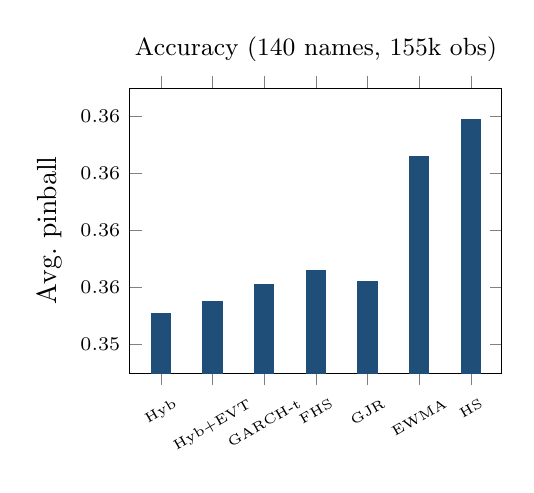
\begin{tikzpicture}
\begin{axis}[width=0.52\textwidth, height=5.2cm, ybar, bar width=7pt,
  symbolic x coords={Hyb, Hyb+EVT, GARCH-t, FHS, GJR, EWMA, HS},
  xtick=data, ymin=0.353, ymax=0.363,
  ylabel={Avg.\ pinball}, x tick label style={font=\tiny, rotate=30},
  tick label style={font=\scriptsize},
  title={\small Accuracy (140 names, 155k obs)}]
\addplot[fill=npblue, draw=npblue] coordinates
  {(Hyb,0.3551) (Hyb+EVT,0.3555) (GARCH-t,0.3561) (FHS,0.3566)
   (GJR,0.3562) (EWMA,0.3606) (HS,0.3619)};
\end{axis}
\end{tikzpicture}\hfill
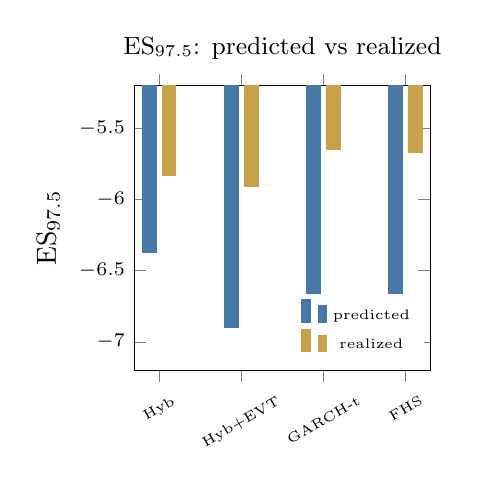
\begin{tikzpicture}
\begin{axis}[width=0.44\textwidth, height=5.2cm, ybar, bar width=5pt,
  symbolic x coords={Hyb, Hyb+EVT, GARCH-t, FHS},
  xtick=data, ymin=-7.2, ymax=-5.2,
  ylabel={ES$_{97.5}$}, x tick label style={font=\tiny, rotate=30},
  tick label style={font=\scriptsize},
  title={\small ES$_{97.5}$: predicted vs realized},
  legend style={font=\tiny, at={(0.98,0.02)}, anchor=south east,
                draw=none}]
\addplot[fill=npmid, draw=npmid] coordinates
  {(Hyb,-6.37) (Hyb+EVT,-6.90) (GARCH-t,-6.69) (FHS,-6.90)};
\addlegendentry{predicted}
\addplot[fill=gold, draw=gold] coordinates
  {(Hyb,-5.83) (Hyb+EVT,-5.91) (GARCH-t,-5.65) (FHS,-5.67)};
\addlegendentry{realized}
\end{axis}
\end{tikzpicture}
\caption{The FRTB battery. Left: average pinball loss by model (axis
truncated to resolve the ordering; differences carry DM 5.2--8.8 vs the
hybrid, all $p \approx 0$); CAViaR, not shown, statistically ties the
hybrid. Right: ES$_{97.5}$ predicted (exact tail integral) vs realized
below each model's own VaR, a model-dependent diagnostic, not a
ranking (every fat-tailed entrant's integral exceeds its own-tail
mean); the joint FZ0 score of the paper is the ranking criterion.}
\label{fig:frtb}
\end{figure}
\clearpage
\begin{figure}[htbp]
\centering
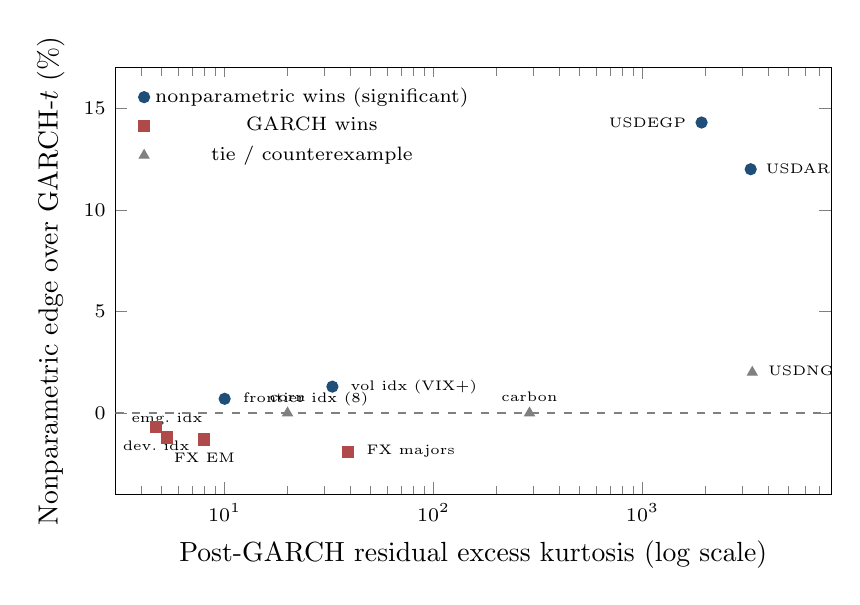
\begin{tikzpicture}
\begin{axis}[width=0.88\textwidth, height=7cm, xmode=log,
  xlabel={Post-GARCH residual excess kurtosis (log scale)},
  ylabel={Nonparametric edge over GARCH-$t$ (\%)},
  ymin=-4, ymax=17, xmin=3, xmax=8000,
  tick label style={font=\scriptsize},
  legend style={font=\scriptsize, at={(0.02,0.98)}, anchor=north west,
                draw=none}]
\addplot[only marks, mark=*, color=npblue] coordinates
  {(10,0.7) (32.8,1.3) (1920,14.3) (3298,12.0)};
\addlegendentry{nonparametric wins (significant)}
\addplot[only marks, mark=square*, color=gred] coordinates
  {(4.7,-0.7) (5.3,-1.2) (8,-1.3) (39,-1.9)};
\addlegendentry{GARCH wins}
\addplot[only marks, mark=triangle*, color=gray] coordinates
  {(20,0) (288,0) (3357,2.0)};
\addlegendentry{tie / counterexample}
\node[font=\tiny, anchor=west] at (axis cs:11,0.7) {frontier idx (8)};
\node[font=\tiny, anchor=west] at (axis cs:36,1.3) {vol idx (VIX+)};
\node[font=\tiny, anchor=east] at (axis cs:1800,14.3) {USDEGP};
\node[font=\tiny, anchor=west] at (axis cs:3500,12.0) {USDARS};
\node[font=\tiny, anchor=north] at (axis cs:4.7,-0.9) {dev.\ idx};
\node[font=\tiny, anchor=south] at (axis cs:5.3,-1.1) {emg.\ idx};
\node[font=\tiny, anchor=north] at (axis cs:8,-1.5) {FX EM};
\node[font=\tiny, anchor=west] at (axis cs:43,-1.9) {FX majors};
\node[font=\tiny, anchor=south] at (axis cs:20,0.1) {corn};
\node[font=\tiny, anchor=south] at (axis cs:288,0.1) {carbon};
\node[font=\tiny, anchor=west] at (axis cs:3600,2.0) {USDNGN (ns)};
\draw[dashed, gray] (axis cs:3,0) -- (axis cs:8000,0);
\end{axis}
\end{tikzpicture}
\caption{The frontier across universes: nonparametric edge vs post-GARCH
residual kurtosis, tier means and single assets with study-reported
kurtosis only (country universe corr 0.53; cross-asset corr 0.43).
The hyperinflation-FX tier (kurtosis $\sim$2000--3300) carries the only
decisive standalone wins; high kurtosis is predictive but neither necessary nor sufficient: carbon (288) and corn (20) tie, and NGN's win is not significant.
The Korea-2026 control (kurtosis 4--13, GARCH wins all 23 assets) sits
in the lower-left regime.}
\label{fig:universes}
\end{figure}
\clearpage
\begin{figure}[htbp]
\centering
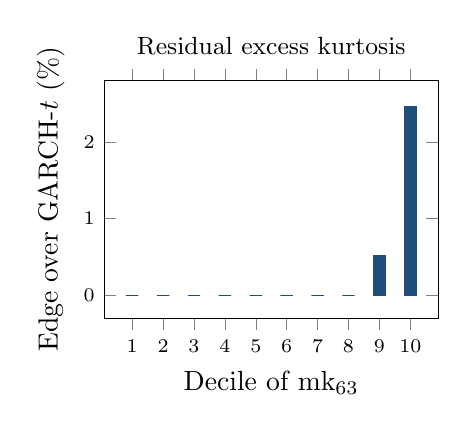
\begin{tikzpicture}
\begin{axis}[width=0.48\textwidth, height=4.6cm, ybar, bar width=4.5pt,
  xlabel={Decile of $\mathrm{mk}_{63}$}, ylabel={Edge over GARCH-$t$ (\%)},
  xtick={1,2,3,4,5,6,7,8,9,10}, ymin=-0.3, ymax=2.8,
  title={\small Residual excess kurtosis}, tick label style={font=\scriptsize}]
\addplot[fill=npblue, draw=npblue] coordinates
  {(1,0)(2,0)(3,0)(4,0)(5,0)(6,0)(7,0)(8,0)(9,0.52)(10,2.46)};
\end{axis}
\end{tikzpicture}\hfill
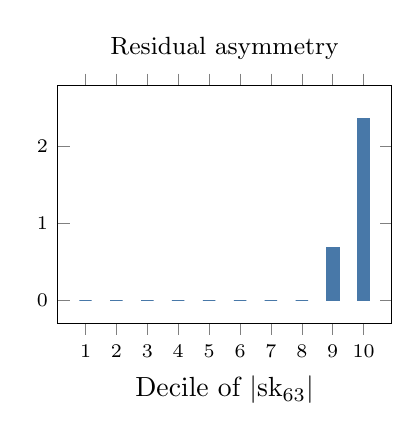
\begin{tikzpicture}
\begin{axis}[width=0.48\textwidth, height=4.6cm, ybar, bar width=4.5pt,
  xlabel={Decile of $|\mathrm{sk}_{63}|$},
  xtick={1,2,3,4,5,6,7,8,9,10}, ymin=-0.3, ymax=2.8,
  title={\small Residual asymmetry}, tick label style={font=\scriptsize}]
\addplot[fill=npmid, draw=npmid] coordinates
  {(1,0)(2,0)(3,0)(4,0)(5,0)(6,0)(7,0)(8,0)(9,0.69)(10,2.37)};
\end{axis}
\end{tikzpicture}
\caption{The misspecification frontier. Nonparametric pinball edge over
GARCH-$t$ by decile of the trailing 63-day residual excess kurtosis
(left) and residual asymmetry (right), 200 CRSP names, 221.6k test
asset-days. Deciles 1--8 are $\approx 0$ (drawn at zero; exact bulk
values in the result file); the edge jumps in the top decile
($+2.46\%$ kurtosis, $+2.37\%$ asymmetry; per-date DM 6.5 in the top
kurtosis decile).}
\label{fig:frontier}
\end{figure}
\clearpage
\section{Supplementary tables}
\begin{table}[htbp]
\centering\small
\begin{threeparttable}
\caption{Summary of the paper's results and scope conditions. Edges are
percentage pinball reductions unless noted; DM statistics are per-date
(conventions note of Section~5 of the paper), one-sided. Panel A: the deployed amortized
residual-hybrid engine (worst case on the accuracy yardstick: no
detectable loss; calm-cell 90\% lower confidence bounds sit above
$-0.25\%$). A separate block reports the direct multi-day
extension, which is not the engine. Panel B: boundary
evidence from configurations not deployed, which motivates the design.}
\label{tab:winloss}
\footnotesize\setlength{\tabcolsep}{3.5pt}
\begin{tabular}{>{\raggedright\arraybackslash}p{0.34\textwidth}>{\raggedright\arraybackslash}p{0.20\textwidth}>{\raggedright\arraybackslash}p{0.38\textwidth}}
\toprule
\multicolumn{3}{l}{\emph{Panel A: the engine}} \\
Result & Magnitude & Significance \\
\midrule
vs GARCH-$t$ / EWMA / HS, $h{=}1$ (avg) & $+0.3$ / $+1.5$ / $+1.9\%$ & DM 4.4--8.3 \\
Top misspecification decile & $+2.7\%$ & DM 6.5 \\
Hyperinflation FX (ARS, EGP) & $+12$--$14\%$ & DM 2.9--3.8 \\
Frontier equity indices (4 of 8) & $\sim$$+1$--$3\%$ & DM 2.1--3.5 \\
2000--2013 frozen-spec holdout (untouched era) & top decile $+0.9\%$ & DM 2.2 (sort); recursive real-time rule $+1.0\%$, DM 2.15; frozen-constant restatement in text \\
Point-in-time universe (Q1-2000 top 200, delistings kept) & top bucket $+2.9\%$; overall $+0.6\%$ & DM 6.6 / 9.0, frozen real-time thresholds \\
Strict calendar splits; annual-refit walk-forward & top decile $+2.5\%$ under all three & DM 6.2 (2020 cut); 3.1 (overall, pre-GFC cut); 6.1 (walk-forward) \\
Familywise error over the $3\times10$ signal-decile grid & 9 cells survive 5\% FWER & Romano--Wolf step-down, incl.\ all three top deciles \\
Exception battery through the 2008 crisis & Kupiec 94\% / Christof.\ 95\% at 99\% & date-clustered $t$ 0.17 at 99\%; at 97.5\%, 0.35 (EVT tail) and $-1.09$ (static overlay, conservative); HS, EWMA fail \\
Joint $(\VaR,\ES)$ FZ0 score, full panel & accuracy layer lowest at both levels & DM 4.8--4.9 vs GARCH-$t$, FHS at 1\%, 5.1 at 2.5\%; 6.2--9.6 vs GAS; static shift concedes 2.5\% (DM $-1.6$), adaptive shift erases it (tie; top-decile cost remains) \\
Cold start / young listings & $+6$--$10\%$ & full-scale panel; no per-asset model applies \\
Calm-quintile edge & $\approx 0$ (point estimates $+0.0$--$+0.2\%$) & bottom-decile 90\% CIs lie above $-0.25\%$; no detectable loss \\
CAViaR (strongest academic rival) & tie (co-best in MCS) & DM 0.4 \\
\midrule
\multicolumn{3}{l}{\emph{Extension (a separate direct multi-day model, not the engine)}} \\
\midrule
Ten-day horizon vs $\sqrt{h}$-scaling & $+1.4\%$ (2014--24) & holds in 2020--22 stress; 2000--13 rerun: tie, DM 0.07 (era-dependent) \\
\midrule
\multicolumn{3}{l}{\emph{Panel B: boundary evidence from configurations not deployed}} \\
\midrule
Bare standalone neural net, single names & $-4.5$ to $-6.2\%$ & DM $+12$ to $+18$; motivates the hybrid design \\
Standalone nonparametric, calm single assets & GARCH as good or better & pooled DM $-9.5$ to $-13.7$; the shape edge needs misspecification \\
Korea 2026 crisis, 23 assets (falsification case) & GARCH wins all & DM $-2.5$ to $-5$; a price crash is not a shape break \\
mk$_{63}$-reweighted FHS (reweighting probe) & worse than plain FHS & DM $-11$ overall and top decile; sharp univariate conditioning collapses the sample \\
Baltic freight; IG credit\tnote{a} & $+15\%$; $+52\%$ & DM 9.6; 30.6; accuracy only, calibration open \\
\bottomrule
\end{tabular}
\begin{tablenotes}\footnotesize
\item[a] Credit and freight fail breach-independence (exceptions
cluster); their entries are accuracy results only. The
credit magnitude is from the FRTB-grade single-asset battery; the
smaller $4\%$ figure in the paper's cross-universe table is from the separate lean hybrid-vs-GARCH sweep, different battery, both reported.
\end{tablenotes}
\end{threeparttable}
\end{table}

\begin{table}[htbp]
\centering
\begin{threeparttable}
\caption{Double sort: the edge needs both a shape break and an active
regime. Cells are the nonparametric-over-GARCH-$t$ pinball edge (\%)
in independent quintiles of the misspecification score (rows) and
trailing volatility (columns), design-era test panel.}
\label{tab:doublesort}
\footnotesize\setlength{\tabcolsep}{5pt}
\begin{tabular}{lccccc}
\toprule
 & rv$_{63}$ Q1 (calm) & Q2 & Q3 & Q4 & Q5 (active) \\
\midrule
mk$_{63}$ Q1 (low) & $+0.24$ & $+0.34$ & $+0.10$ & $+0.01$ & $-0.14$ \\
Q2 & $+0.16$ & $+0.20$ & $+0.22$ & $+0.09$ & $-0.57$ \\
Q3 & $-0.02$ & $+0.19$ & $+0.25$ & $+0.44$ & $+0.04$ \\
Q4 & $+0.08$ & $+0.15$ & $+0.35$ & $+0.23$ & $+0.10$ \\
Q5 (high) & $-0.10$ & $+0.44$ & $+0.68$ & $+0.61$ & $\mathbf{+2.33}$ \\
\bottomrule
\end{tabular}
\begin{tablenotes}\footnotesize
\item Top-row date-clustered DM by volatility quintile: 0.7, 2.3, 1.2,
2.8, 6.4. The bottom-left and top-right regions are the point:
neither ingredient alone produces the concentration.
\end{tablenotes}
\end{threeparttable}
\end{table}
\begin{table}[htbp]
\centering\small
\caption{Model selection by task and regime.
Each row is established in the section cited.}
\label{tab:decision}
\begin{tabular}{p{0.44\textwidth}p{0.30\textwidth}l}
\toprule
Task / regime & Winner & Where \\
\midrule
Point quantile accuracy, tabular state & GBM (trees) & Section~3.2 of the paper \\
Single asset, calm ($\sim$90\% of asset-days) & GARCH-$t$ & Section~5 of the paper \\
Single asset, top misspecification decile & Nonparametric ($+2.7\%$, DM 6.5) & Section~5 of the paper \\
Amortized cross-name panel, any regime & Nonparametric always; no gate & Section~5.4 of the paper \\
Regulatory ES with a $\ge$GARCH floor & Residual-hybrid $+$ EVT $+$ conformal & Section~6 of the paper \\
\bottomrule
\end{tabular}
\end{table}

\begin{table}[htbp]
\centering
\begin{threeparttable}
\caption{Cross-universe multiplicity: Holm step-down over all 93
instrument-level comparisons in the three exploratory universes of the
paper's cross-universe table (24 FX pairs, 26 country indices, 43
cross-asset instruments). One-sided $p$ from each instrument's date-clustered DM
statistic; familywise $\alpha=5\%$. Ranks below twelve all have
$p>0.02$ and are omitted.}
\label{tab:holm}
\footnotesize\setlength{\tabcolsep}{5pt}
\begin{tabular}{rllcccl}
\toprule
Rank & Instrument & Universe & DM & $p$ (one-sided) & Holm cutoff & Verdict \\
\midrule
1 & PJM power\tnote{a} & cross-asset & 283.1 & $<10^{-16}$ & $5.38\times10^{-4}$ & artifact\tnote{a} \\
2 & Baltic Dry & cross-asset & 9.36 & $<10^{-16}$ & $5.43\times10^{-4}$ & survives \\
3 & VIX & cross-asset & 5.71 & $5.7\times10^{-9}$ & $5.49\times10^{-4}$ & survives \\
4 & V2X & cross-asset & 5.03 & $2.5\times10^{-7}$ & $5.56\times10^{-4}$ & survives \\
5 & VVIX & cross-asset & 4.66 & $1.6\times10^{-6}$ & $5.62\times10^{-4}$ & survives \\
6 & USDEGP & FX & 3.80 & $7.2\times10^{-5}$ & $5.68\times10^{-4}$ & survives \\
7 & Kenya NSE20 & indices & 3.52 & $2.2\times10^{-4}$ & $5.75\times10^{-4}$ & survives \\
8 & Wheat & cross-asset & 3.51 & $2.2\times10^{-4}$ & $5.81\times10^{-4}$ & survives \\
9 & MOVE & cross-asset & 3.22 & $6.4\times10^{-4}$ & $5.88\times10^{-4}$ & fails \\
10 & Sri Lanka CSEALL & indices & 3.20 & $6.9\times10^{-4}$ & $5.95\times10^{-4}$ & fails \\
11 & Gasoline & cross-asset & 3.20 & $6.9\times10^{-4}$ & $6.02\times10^{-4}$ & fails \\
12 & USDARS & FX & 2.86 & $2.1\times10^{-3}$ & $6.10\times10^{-4}$ & fails \\
\bottomrule
\end{tabular}
\begin{tablenotes}\footnotesize
\item The family is every instrument-level look in the three
exploratory universes; the Korea-2026 falsification case (23 assets,
GARCH-$t$ wins throughout) is not part of the win family. Bonferroni
at $0.05/93$ gives the identical survivor set. The pooled crisis-FX
comparison (DM 4.12, $p\approx1.9\times10^{-5}$) and the
kurtosis--edge correlations (0.53 across indices, 0.43 cross-asset)
are pooled and gradient statistics outside this instrument-level
family; they are the replication evidence the paper's cross-universe
claims rest on.
\item[a] Retained in the family because the raw sweep contains it,
but not a win: the paper's cross-asset audit reclassifies electricity
as a log-return artifact on near-zero and negative prices, refit on price differences, GARCH wins PJM (DM $-2.73$), so the survivor count the text quotes is seven.
\end{tablenotes}
\end{threeparttable}
\end{table}

\subsection*{Direct expected-shortfall backtests}\label{sec:esbt-oa}
Exception counts test the VaR level; they do not test ES. The main text adds two
direct ES \emph{calibration} backtests: the McNeil--Frey (2000)
exceedance-residual test, whose statistic is the mean standardized loss beyond
VaR, zero under a correct ES \citep{mcneilfrey2000}; and the Acerbi--Sz\'ekely
(2014) statistic $Z_2$, negative when ES understates the realized tail
\citep{acerbi2014backtesting}. These complement the jointly consistent FZ0 loss
used for forecast comparison; \citet{noldeziegel2017elicitability} and
\citet{bayer2022esr} draw the distinction between backtesting the calibration of
an ES forecast and comparing forecasts through a jointly consistent score.
Table~\ref{tab:esbt} reports the two calibration tests on the pooled panel (140
CRSP names, per-name GARCH-$t$ fit on the first $60\%$, evaluated on the held-out
$40\%$; $155{,}120$ asset-day observations across $1{,}108$ test dates), with
inference clustered by calendar date. Gaussian innovations are decisively
inadequate in this daily-data battery: the Gaussian filter is worst on every ES
metric, its mean exceedance residual reaching $-0.78$ standard deviations at the
$1\%$ level ($Z_2=-1.07$). Among the fat-tailed entrants no model dominates every
diagnostic. The EVT-tailed engine carries the $Z_2$ closest to zero at both
levels and is the only entrant not rejected by the $1\%$ Kupiec exception test;
at $2.5\%$ it and FHS are the only models McNeil--Frey does not reject (engine
mean exceedance residual $-0.02$, $p=0.49$), while GARCH-$t$ and the Gaussian
filter are. The limitation is the $1\%$ tail: there every model's mean exceedance
residual is significantly negative, the engine included, and FHS's is marginally
closer to zero than the engine's ($-0.19$ against $-0.24$), though both are
rejected. The message is consistent with the exception tests and the joint
score: fat-tailed specifications materially improve tail calibration, the
engine's tail is the best calibrated overall, and the $1\%$ tail on large caps
leaves room that no daily model here closes.

\begin{table}[t]
\centering
\begin{threeparttable}
\caption{Direct expected-shortfall backtests. 140 CRSP names, pooled test
panel. Breach is the realized exception rate (target $\alpha$); Kupiec $p$ is
the unconditional-coverage test. $Z_2$ is the Acerbi--Sz\'ekely (2014)
statistic, negative when ES understates the tail. MF is the McNeil--Frey (2000)
mean exceedance residual (standardized loss beyond VaR, zero under correct ES)
with its bootstrap $p$.}
\label{tab:esbt}
\small\setlength{\tabcolsep}{5pt}
\begin{tabular}{lcccc|cccc}
\toprule
 & \multicolumn{4}{c}{$\alpha=2.5\%$} & \multicolumn{4}{c}{$\alpha=1\%$}\\
\cmidrule(lr){2-5}\cmidrule(lr){6-9}
Model & Breach & Kupiec\,$p$ & $Z_2$ & MF ($p$) & Breach & Kupiec\,$p$ & $Z_2$ & MF ($p$) \\
\midrule
GARCH-normal & $0.027$ & $0.00$ & $-0.36$ & $-0.56\,(0.00)$ & $0.016$ & $0.00$ & $-1.07$ & $-0.78\,(0.00)$ \\
GARCH-$t$ & $0.028$ & $0.00$ & $-0.14$ & $-0.07\,(0.00)$ & $0.011$ & $0.03$ & $-0.14$ & $-0.29\,(0.00)$ \\
GARCH-FHS & $0.028$ & $0.00$ & $-0.14$ & $-0.02\,(0.39)$ & $0.011$ & $0.00$ & $-0.18$ & $-0.19\,(0.00)$ \\
Engine (hybrid$+$EVT) & $0.028$ & $0.00$ & $\mathbf{-0.12}$ & $\mathbf{-0.02\,(0.49)}$ & $0.010$ & $\mathbf{0.12}$ & $\mathbf{-0.12}$ & $-0.24\,(0.00)$ \\
\bottomrule
\end{tabular}
\begin{tablenotes}\footnotesize
\item Inference for the McNeil--Frey and $Z_2$ $p$-values clusters on the
$1{,}108$ trading dates rather than treating the $155{,}120$ asset-days as
independent, since the $140$ names share within-day market shocks. Kupiec is the
analytic unconditional-coverage test. Source: \texttt{es\_backtests\_results.json}.
\end{tablenotes}
\end{threeparttable}
\end{table}

\subsection*{Realized measures and the scale--shape decomposition}\label{sec:rgarch-oa}
The main-text battery reads only daily returns, the regime the estimator is built
for. To place it against a method that reads intraday data, and to ask what the
misspecification frontier is made of, we build five-minute realized measures from
TAQ for thirty large-capitalization U.S.\ equities over 2014--2024 (realized
variance is the sum of squared five-minute log-returns, cleaned by regular sale
conditions, a daily price band, and a $20\%$ return clip) and fit a Realized GARCH
\citep{hansen2012realized}: the log-linear conditional variance
$\log h_t=\omega+\beta\log h_{t-1}+\gamma\log \mathrm{RV}_{t-1}$ with a measurement
equation $\log\mathrm{RV}_t=\xi+\phi\log h_t+\tau(z_t)+u_t$ linking the realized
measure to the latent variance, estimated jointly by Gaussian quasi-maximum
likelihood. Table~\ref{tab:rgarch} reports the result on 1{,}108 common test dates.
Two facts follow. The realized scale lowers FZ0 well below the daily-data accuracy
core at both levels (DM $6.0$ at 2.5\%, $4.5$ at 1\%): intraday information prices
volatility more sharply than any daily filter. But the gain is scale, not shape.
Holding the realized scale fixed and re-fitting the pooled state-conditioned
residual-quantile learner, the EVT tail, and the misspecification score on the
realized residuals moves FZ0 within noise, in magnitude below one Diebold--Mariano
standard error overall and in the top realized-residual score decile (the top three
deciles reach DM $-1.4$ at $1\%$, directional but not significant). On these
large-capitalization names a realized scale absorbs most of what the score detects
on daily-GARCH residuals, so on the intraday-covered segment the two are
substitutes; the score's distinctive value is in the daily-data regime and the
cross-asset and day-one settings where a realized scale does not exist.

\begin{table}[t]
\centering
\begin{threeparttable}
\caption{The scale--shape decomposition. Thirty large-cap U.S.\ equities, 2014--2024
(1{,}108 test dates), joint $(\VaR,\ES)$ FZ0 loss (lower is better) at both FRTB
levels. The scale is a proper Realized GARCH except in the first row (the daily-data
accuracy core). DM is date-clustered (Newey--West, 5 lags) against the realized scale
with an unconditional residual quantile; a positive DM is worse than that benchmark.}
\label{tab:rgarch}
\small\setlength{\tabcolsep}{6pt}
\begin{tabular}{lcccc}
\toprule
Model & FZ0 $2.5\%$ & DM & FZ0 $1\%$ & DM \\
\midrule
Daily core (GARCH-$t$ $+$ EVT) & $1.501$ & $+6.0$ & $1.774$ & $+4.5$ \\
Realized scale $+$ residual quantile & $1.446$ & --- & $1.737$ & --- \\
\quad $+$ EVT tail & $1.446$ & $-0.2$ & $1.740$ & $+1.4$ \\
\quad $+$ pooled shape learner & $1.445$ & $-0.2$ & $1.739$ & $+0.3$ \\
\quad $+$ shape $+$ EVT (realized-hybrid) & $1.446$ & $+0.1$ & $1.736$ & $-0.3$ \\
\bottomrule
\end{tabular}
\begin{tablenotes}\footnotesize
\item The daily core's DM is against the realized benchmark (the intraday-scale gain).
The pooled shape learner is the paper's state-conditioned residual-quantile model,
retrained on the realized-scale residuals. Returns are CRSP daily; the intersection is
common across models. Source: \texttt{rgarch\_bench\_results.json},
\texttt{realized\_hybrid\_results.json}.
\end{tablenotes}
\end{threeparttable}
\end{table}

\clearpage
\section{The two-regime example}
\subsection*{A synthetic boundary check: when the frontier does
\emph{not} appear}\label{sec:toy}

Before the real data, a simulation with known truth (run once, seed
fixed) checks the formal results and, more usefully, delineates when
the frontier edge should \emph{fail} to appear. The data-generating
process is deliberately favorable to the score: unit-variance
Student-$t$ residuals whose degrees of freedom switch between a calm
regime ($\nu=12$) and a fat regime ($\nu=3$) under a persistent Markov
chain; forecasters see the trailing 63-day kurtosis score and compete
at $\tau \in \{0.01, 0.025\}$ (80{,}000 days; scale known, isolating
shape). First, the Lemma~1 of the paper identity
verifies numerically: the regret integral and the Monte-Carlo regret
agree to five decimals ($3.5\times10^{-5}$ at $\tau=0.01$). Second, the
conformal shift moves realized coverage toward nominal on the held-out
split, as Proposition~1 of the paper promises. Third, and most instructive, the score-binned nonparametric
forecaster does
\emph{not} beat the fixed shape here: a single $t_{\widehat\nu}$
fitted on the mixture ($\widehat\nu = 6.8$) is nearly unbeatable at
these levels, with total regret under $0.5\%$ and no decile gradient.
Two mechanisms explain it, and both teach. (i)~By
Lemma~1 of the paper regret is \emph{quadratic} in the quantile
wedge, and at $\tau \ge 0.01$ the wedge between the fitted compromise
and either regime is small; static kurtosis \emph{blending} is a
second-order sin. (ii)~The sample kurtosis of a $t_\nu$ law is a noisy statistic when
tails are fat: its usual moment-based asymptotic variance requires a
finite eighth moment ($\nu>8$), and the population kurtosis itself does
not exist for $\nu\le4$, so sixty-three observations cannot reliably
rank regimes that differ only in a static $\nu$. The jump and
asymmetry signals, whose top deciles independently survive familywise
control, corroborate the ordering, and a tail-index (Hill-type)
variant of the score is an obvious robustness extension. For the empirical sections this means the real-data top-decile edge of Section~5 of the paper
cannot be an artifact of stationary fat tails being averaged over
(that configuration is the one the simulation shows a fixed shape
handles) and is consistent with \emph{local} shape breaks a single
fitted $\nu$ cannot straddle: asymmetry, jump clustering, and residual misfit
that co-move with the score. This is the same conclusion the Korea 2026
falsification case reaches from the opposite direction (price crashes
are not residual misspecification), and it is why the score combines
kurtosis with asymmetry and a jump indicator rather than kurtosis
alone. (Simulation script \texttt{toy\_example.py} ships with the code
release.)


\section{Trading implications and scenario generation}
\textbf{Trading implications.} The universes where the nonparametric tail wins (crisis FX, volatility indices, credit spreads, frontier equities) are the desks where tail-shape-aware
sizing and hedging matter most. The \emph{direction} of the trade matters
as much as its location: a correct physical-measure tail forecast
does not by itself make bought crash insurance profitable, because the
crash risk premium can survive conditioning on a correct forecast.
The application the evidence supports is the opposite side, selling tail
protection, where the model supplies tail control rather than alpha on
the mean. The gating experiment provides no evidence that the score times
individual crash days, so its role there is continuous tail-risk
measurement, not a market-timing signal.

\textbf{Scenario generation.} Because the shape stage carries an exact
inverse-CDF sampler, calibrating intractable scenario generators
(rough volatility, Hawkes, jump-diffusions) for CCAR/ICAAP-style
stress design is a natural extension; it is not developed here.


%% ===== CONCLUSION =====

\clearpage
\section{Proofs}\label{app:proofs}

The four formal results of Section~3.3 of the paper are stated with
proof sketches in the body; the complete arguments, with all regularity
hypotheses made explicit, are collected here. Throughout, $\rho_\tau(u)
= u(\tau - \mathbb{I}\{u<0\})$ and $q_F = F^{-1}(\tau) = \inf\{x:F(x)\ge
\tau\}$ is the lower generalized inverse.

\subsection*{Proof of Lemma~1 of the paper (pinball regret identity)}

Assume $\mathbb{E}|Z|<\infty$, so
\[
S(q) = (1-\tau)\!\int_{(-\infty,q]}\!(q-z)\,dF(z)
\;+\; \tau\!\int_{(q,\infty)}\!(z-q)\,dF(z)
\]
is finite for every $q$, and $S$ is convex (an expectation of the
convex maps $q\mapsto\rho_\tau(z-q)$). For fixed $z$, $q\mapsto
\rho_\tau(z-q)$ is Lipschitz with constant $\max(\tau,1-\tau)$, so the
difference quotients $[\rho_\tau(Z-q')-\rho_\tau(Z-q)]/(q'-q)$ are
bounded by the integrable constant $\max(\tau,1-\tau)$; dominated
convergence justifies differentiating under the expectation wherever the
one-sided limits exist. Off the atoms of $F$,
\[
\frac{d}{dq}\,\rho_\tau(z-q) = \mathbb{I}\{z<q\}-\tau ,
\qquad\Longrightarrow\qquad
S'(q) = \mathbb{E}\,\mathbb{I}\{Z<q\}-\tau = F(q^-)-\tau,
\]
which equals $F(q)-\tau$ for all but countably many $q$. Since $S$ is
convex, hence absolutely continuous, the fundamental theorem of
calculus gives
\[
S(q)-S(q_F)=\int_{q_F}^{q}\big(F(u)-\tau\big)\,du,
\]
the countable atom set being Lebesgue-null; \emph{no continuity
hypothesis on $F$ is needed for this identity}. For nonnegativity,
note $q_F=\inf\{x:F(x)\ge\tau\}$ implies $F(u)\ge\tau$ for $u\ge q_F$
and $F(u)<\tau$ for $u<q_F$. If $q>q_F$ the integrand is $\ge0$ on
$[q_F,q]$, so the integral is $\ge0$; if $q<q_F$,
\[
S(q)-S(q_F)=\int_{q_F}^{q}\big(F(u)-\tau\big)\,du
=\int_{q}^{q_F}\big(\tau-F(u)\big)\,du\;\ge\;0 ,
\]
the integrand again $\ge0$ on $[q,q_F]$. Equality holds iff $F(u)=\tau$
for Lebesgue-a.e.\ $u$ between $q_F$ and $q$. Finally, if $F$ is
absolutely continuous with density $0<m\le f\le M$ on the interval
joining $q_F$ and $q$, then $F$ is continuous there, so $F(q_F)=\tau$
and $F(u)-\tau=\int_{q_F}^{u}f$; hence $m|u-q_F|\le|F(u)-\tau|\le
M|u-q_F|$, and integrating over the interval yields
$\tfrac{m}{2}(q-q_F)^2\le S(q)-S(q_F)\le\tfrac{M}{2}(q-q_F)^2$.
\hfill$\square$

\subsection*{Proof of Proposition~1 of the paper (split-conformal
validity)}

Let $k=\lceil(n{+}1)\tau\rceil$ and assume $1\le k\le n$ so that the
$k$-th order statistic $e_{(k)}=c_\tau$ of the $n$ calibration errors
$\{e_1,\dots,e_n\}$ exists; when $k=n+1$ (i.e.\ $\tau$ within $1/(n+1)$
of $1$) set $c_\tau=+\infty$, giving coverage $1$. Suppose the $n+1$
errors $e_1,\dots,e_{n+1}$ (calibration plus the test error
$e_{n+1}=z_{n+1}-\widehat q(\tau\mid s_{n+1})$) are exchangeable and
almost surely distinct. Then the rank $R$ of $e_{n+1}$ among the pooled
$n+1$ values is uniformly distributed on $\{1,\dots,n+1\}$. By
construction $\widetilde q(\tau\mid s_{n+1})=\widehat q(\tau\mid
s_{n+1})+c_\tau$, so
\[
\{z_{n+1}\le\widetilde q(\tau\mid s_{n+1})\}
=\{e_{n+1}\le c_\tau\}
=\{e_{n+1}\le e_{(k)}\}
=\{R\le k\},
\]
the middle equality using a.s.\ distinctness (with ties the middle
equality fails; e.g.\ if all $e_i$ are equal the event has probability
$1$, which can exceed the stated upper bound). Therefore
\[
\Pr\big(z_{n+1}\le\widetilde q(\tau\mid s_{n+1})\big)
=\Pr(R\le k)=\frac{k}{n+1}
=\frac{\lceil(n{+}1)\tau\rceil}{n+1}.
\]
Since $(n{+}1)\tau\le\lceil(n{+}1)\tau\rceil<(n{+}1)\tau+1$, dividing by
$n+1$ gives $\tau\le k/(n+1)<\tau+\tfrac1{n+1}$. The probability is over
the joint law of calibration and test points; the guarantee is
marginal, not conditional on $s_{n+1}$, because a single scalar shift
$c_\tau$ pooled across states cannot deliver state-conditional
coverage. \hfill$\square$

\subsection*{Proof of Proposition~2 of the paper (tail wedge)}

Fix $\nu>2$, so the $t_\nu$ law has finite variance and its
unit-variance version $Z=T_\nu\sqrt{(\nu-2)/\nu}$ is well defined. The
$t_\nu$ density is $\sim C_\nu|x|^{-(\nu+1)}$ as $|x|\to\infty$, so the
lower tail is regularly varying with index $-\nu$: $\Pr(T_\nu<-x)=
\tilde c_\nu x^{-\nu}(1+o(1))$. Unit-variance scaling multiplies the
constant, $\Pr(Z<-x)=c_\nu x^{-\nu}(1+o(1))$ with
$c_\nu=\tilde c_\nu((\nu-2)/\nu)^{\nu/2}$, and leaves the index $\nu$
unchanged. Writing $U(\tau)=|Q_\nu(\tau)|$ and inverting the regularly
varying tail \citep{embrechts1997} gives $\tau=c_\nu U(\tau)^{-\nu}
(1+o(1))$, hence $U(\tau)=(c_\nu/\tau)^{1/\nu}(1+o(1))$ as
$\tau\downarrow0$, i.e.\ $Q_\nu(\tau)=-(c_\nu/\tau)^{1/\nu}(1+o(1))$.
For $\nu_1<\nu_2$,
\[
\frac{|Q_{\nu_1}(\tau)|}{|Q_{\nu_2}(\tau)|}
=\frac{(c_{\nu_1}/\tau)^{1/\nu_1}}{(c_{\nu_2}/\tau)^{1/\nu_2}}\,(1+o(1))
=\text{const}\cdot\tau^{-(1/\nu_1-1/\nu_2)}(1+o(1))\;\longrightarrow\;\infty
\]
because $1/\nu_1>1/\nu_2$. Thus for all sufficiently small $\tau$ both
quantiles are negative with $|Q_{\nu_1}(\tau)|>|Q_{\nu_2}(\tau)|$, i.e.\
$Q_{\nu_1}(\tau)<Q_{\nu_2}(\tau)$, and the wedge
$|Q_{\nu_1}(\tau)-Q_{\nu_2}(\tau)|\to\infty$. The ordering therefore
holds for every $\tau<\delta$ for some $\delta>0$; putting
$\tau^*=\min(\delta,\tfrac12)$ gives $\tau^*\in(0,\tfrac12)$ as
asserted. (This establishes \emph{existence} of $\tau^*$; the actual
crossover $\tau_c$ where the ordering flips is not claimed here and is
located numerically in the crossover remark of the paper.) Under local truth
$t_{\nu_1}$, applying the corresponding equation of the paper with $q=Q_{\nu_2}(\tau)$ and
$q_F=Q_{\nu_1}(\tau)$ bounds the regret below by
$\tfrac{m}{2}(Q_{\nu_1}(\tau)-Q_{\nu_2}(\tau))^2$, with $m$ the minimum
of the $t_{\nu_1}$ density on the wedge interval. \hfill$\square$

\subsection*{On the score-ordering: why it is an empirical regularity, not a theorem}
We state the score-ordering as an empirical regularity rather than a
theorem, and record here why no clean monotonicity theorem holds at the
deployable levels. The tail-wedge result (Proposition~2 of the paper)
orders a given pair of Student-$t$ tail indices only below a pair-specific
crossover level $\tau^*(\nu_1,\nu_2)$; it does not deliver monotonicity of
the wedge in the tail index at a fixed operational $\tau$. More
fundamentally, the innovations are unit-variance by construction, and for
the unit-variance $t_\nu$ the level-$\tau$ quantile is
$Q_\nu(\tau)=\sqrt{(\nu-2)/\nu}\;t_\nu^{-1}(\tau)$, which is \emph{not}
monotone in $\nu$: as $\nu\downarrow2$ the normalization
$\sqrt{(\nu-2)/\nu}\to0$ pulls the fixed-$\tau$ quantile back toward zero,
so an arbitrarily heavy-tailed unit-variance $t$ eventually has a
fixed-$\tau$ quantile arbitrarily close to the center rather than far into
the tail. The non-monotonicity is already active at the regulatory levels:
at $\tau=0.025$, $Q_5(0.025)\approx-1.99$ is \emph{less} extreme than
$Q_8(0.025)\approx-2.00$, so a heavier-tailed standardized $t$ carries the
less extreme $2.5\%$ quantile. A clean ordering theorem would therefore
have to restrict the tail index to an explicit interval, isolate a range
of $\tau$ on which $\partial Q_\nu(\tau)/\partial\nu$ has one sign, and
control the density factor in the regret expansion; we do not pursue that
narrow statement. The exact content we retain is the regret identity
(Lemma~1 of the paper) and the tail-wedge ordering (Proposition~2 of the
paper), and the frontier itself is documented empirically in the paper.
\hfill$\square$



\begin{spacing}{1.0}
\bibliographystyle{plainnat}
\bibliography{refs_v3}
\end{spacing}

\subsection*{Proof of Lemma~2 of the paper (generative sampler)}
Let $\widetilde{q}(\cdot \mid s)$ be nondecreasing and left-continuous
on $(0,1)$ and $\tau \sim U(0,1)$, and set
$Z^*=\widetilde q(\tau\mid s)$ and
$G(x)=\sup\{t\in(0,1):\widetilde q(t\mid s)\le x\}$ (with
$\sup\emptyset=0$). Monotonicity makes
$\{t:\widetilde q(t\mid s)\le x\}$ an interval with left endpoint $0$,
and left-continuity ensures the supremum is attained when the set is
nonempty, so the set equals $(0,G(x)]$; hence
$\{Z^*\le x\}=\{\tau\le G(x)\}$ and
$\Pr(Z^*\le x)=G(x)$, i.e.\ $Z^*$ has CDF $G$. Because $G$ so defined
is the upper generalized inverse of $\widetilde q$, and a
left-continuous nondecreasing $\widetilde q$ is in turn the lower
generalized inverse of $G$, the quantile function of $Z^*$ is exactly
$\widetilde q(\cdot\mid s)$. When $\widetilde q$ is an estimated curve,
the argument applies verbatim to the estimate: the sampler is exact for
the \emph{fitted} conditional law, which is the claim. $\square$

\end{document}
